
\documentclass[conference]{IEEEtran}

\IEEEoverridecommandlockouts
\usepackage{graphicx}

\usepackage[bitstream-charter]{mathdesign}
\usepackage[utf8]{inputenc}
\usepackage[T1]{fontenc}

\usepackage{amsmath, graphicx, setspace}

\usepackage[lofdepth,lotdepth]{subfig}
\usepackage[justification=centering, labelsep=space, figurewithin=none, tablewithin=none, labelfont=bf]{caption}
\usepackage{multirow}
\usepackage{array}

\hyphenchar\font=-1
\sloppy


\begin{document}

\title{CLOUD DETECTION IN SATELLITE IMAGES}


\author{
    \IEEEauthorblockN{Şevval Bulburu, Mehmet Alperen Ölçer}
    \IEEEauthorblockA{  Bilgisayar Mühendisliği Bölümü\\
                        Yıldız Teknik Üniversitesi, 34220 Istanbul,  Türkiye\\
                        \{sevval.bulburu, alperen.olcer\}@yildiz.edu.tr }
}

\maketitle

\begin{ozet}
İnsanoğlu, doğayı anlama ve açıklama çabası içerisinde olmuştur ve teknolojideki ilerlemeler sayesinde hava olayları tahmin edilebilir hale gelmiştir. Bu başarı büyük ölçüde bulutların hareketlerinin takip edilmesiyle mümkün olmaktadır. Bulut tespiti, uydu görüntülerindeki bulutların tespit edilmesi ve analiz edilmesi için görüntü işleme teknolojisinden yararlanmaktadır. Bu yöntem meteoroloji, çevre izleme, tarım, ormancılık, kent planlaması, askeri istihbarat gibi birçok alanda kullanılmaktadır. Bulut tespit teknolojisi, uydu fotoğraflarını analiz eden yazılımlar aracılığıyla bulut yoğunluğu, yükseklik, boyut, hareket ve tür gibi özellikleri değerlendirerek veri toplamayı mümkün kılmaktadır. Bazı durumlarda uydu görüntüleme çalışmaları yeryüzünden toplanan verilerle gerçekleştirilmektedir. Fakat atmosferdeki bulutlar, yeryüzü ile uydu arasında yer aldığında bu çalışmalara verimlilik açısından zorluklar yaratmaktadır. Bu araştırmanın temel amacı, bu gibi sorunları çözmek ve bulut tespitin uygulamalarda kullanımını mümkün kılmaktır. Bu zorluğun üstesinden gelmek için U-Net mimarisi kullanılarak bir model oluşturulmuştur. Eğitim sonucunda elde edilen \%91 başarı oranı, modelin performansının bir ölçüsü olarak değerlendirilmektedir.
%\boldmath
\end{ozet}
\begin{IEEEanahtar}
Bulut tespiti, Görüntü işleme, Uydu görüntüleri, Meteoroloji, Çevre izleme, Veri toplama, U-Net mimarisi, semantik segmentasyon, Landsat 8.
\end{IEEEanahtar}

\begin{abstract}

Throughout history, humans have strived to comprehend and explain nature and advancements in technology now allow for weather forecasting by tracking clouds. Cloud detection, employing image processing technology, is widely utilized across various fields such as meteorology, environmental monitoring, agriculture, forestry, urban planning, and military intelligence. Software-based cloud detection scans satellite images to analyze cloud properties including density, height, size, movement, and type, facilitating data collection for purposes like environmental monitoring and disaster management. However, when clouds obstruct the view between the surface and satellite, satellite imagery studies face efficiency challenges. This research aims to overcome such obstacles by adopting the U-Net architecture. With an impressive accuracy of \%91 achieved through training, the model's performance can be deemed successful.
%\boldmath
\end{abstract}
\begin{IEEEkeywords}
Cloud detection, Image processing, satellite imagery, meteorology, environmental monitoring, data collection, U-Net architecture, semantic segmentation,  Landsat 8.
\end{IEEEkeywords}


\section{Introduction}

Clouds, being condensed atmospheric water vapor, serve vital roles like rain provision, but also obstruct the examination of the Earth's surface via satellite imagery, necessitating their detection and removal for most remote sensing applications. This importance was underscored by the inability to capture real-time images after the Kahramanmaras earthquake in 2023 due to dust and snowfall clouds. Researchers have utilized various satellite data sources, including MODIS, GOSAT, Landsat-8, France's Sentinel-1/2 satellites, Europe's Spot series, FY2G, GaoFen-1, and geostationary weather satellites to study atmospheric phenomena. However, cloud detection is challenging due to varying cloud patterns and their overlap with other features, different optical properties, and resemblance to other meteorological phenomena. This project offers a solution, employing semantic segmentation based on U-Net for cloud detection, and a model trained on Landsat-8 data was developed to handle such extreme cases.

\section{Preliminary Examination}
The report explores the development of a cloud detection algorithm from satellite images, crucial for weather forecasting, emergency management, and climate research. The project employs machine learning models and image processing techniques for cloud detection, specifically using semantic segmentation and remote sensing through the U-Net architecture, with satellite images sourced from the Landsat-8 dataset.

\subsection{Literature Review}

Cloud detection algorithm research, which likely began in the 1990s, has seen considerable advancements. \cite{first} In a 2017 study, a deep learning model was built to distinguish cloud and snow using convolutional neural networks and a multiscale prediction technique, achieving precision, recall, and mIOU of 92.4, 91.5, and 90.6 respectively. \cite{second} A 2018 study focused on small and thin cloud detection, employing an NSS and Gabor featured model with a precision and recall of 91.61 and 86.39. \cite{third} In 2019, a study used a CNN (Convolutional Neural Network ) based on segNet, improving overall accuracies to 95.26 and 95.47 for Landsat 7 and 8 images. \cite{fourth} Another 2019 study sought to prevent incorrect cloud detection in snowy areas using the RS-Net model, achieving an accuracy and F1 score of 94.54 and 85.59. \cite{fifth} In 2021, a study employed U-Net on Landsat 8 images, achieving precision and recall values of 85.28 and 83.23.
\newpage
The abstracts of the all researches are given below at Figure \ref{lit_rew}.
\begin{figure}[htp]
    \centering
    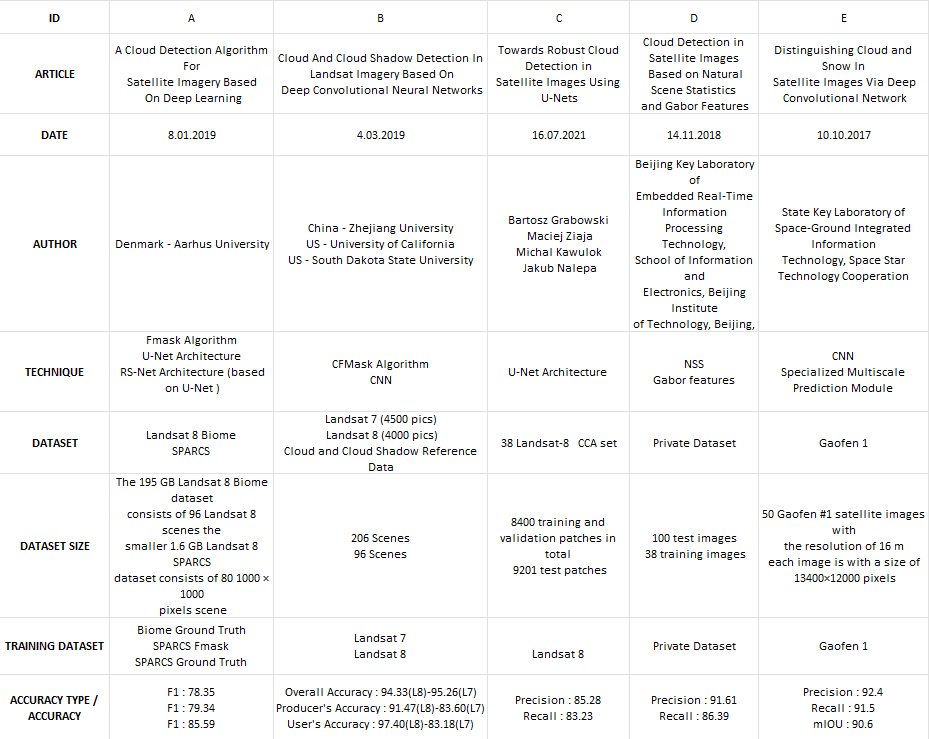
\includegraphics[scale=0.3]{images/litareture.png}
    \caption{Abstracts of All Researches}
    \label{lit_rew}
\end{figure}

A: \cite{first}, B: \cite{second}, C: \cite{third}, D: \cite{fourth}, E: \cite{fifth}
\\
\section{System Design}
The goal of this project is to develop a model for cloud detection based on U-Net architecture employing semantic segmentation.

\subsection{Dataset Design}

The model's training utilized Landsat 8 satellite images, with the L8 dataset consisting of 38 scenes divided into 384x384 pixel patches. For training purposes, 8,400 patches were created, while 9,200 patches were designated for testing. Each patch comprised four spectral channels: Red, Green, Blue, and Near Infrared. Notably, the dataset did not include combined channels.

To assess the dataset's suitability for model evaluation, the patches were examined to identify any significant geographical challenges. Patches from different channels were merged into single patches and thoroughly evaluated, confirming the dataset's appropriateness for model training.

All channelized images were combined and processed to generate a model-compatible dataset, stored in a location referred to as the "hub." This storage approach facilitates easy utilization of the dataset in any Python environment.

The dataset includes unchallenging and challenging images for training and testing of the model. Examples of unchallenging images are given below Figure \ref{easy} while challenging images are provided below Figure \ref{hard}. 
\begin{figure}[!htbp]
    \centering
    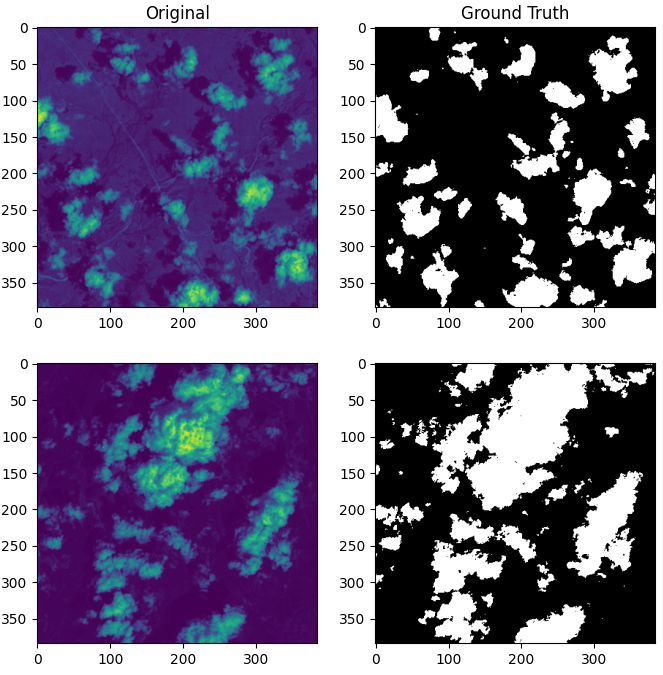
\includegraphics[scale=0.3]{images/easy.png}
    \caption{Example for unchallenging train images}
    \label{easy}
\end{figure}

\begin{figure}[!htbp]
    \centering
    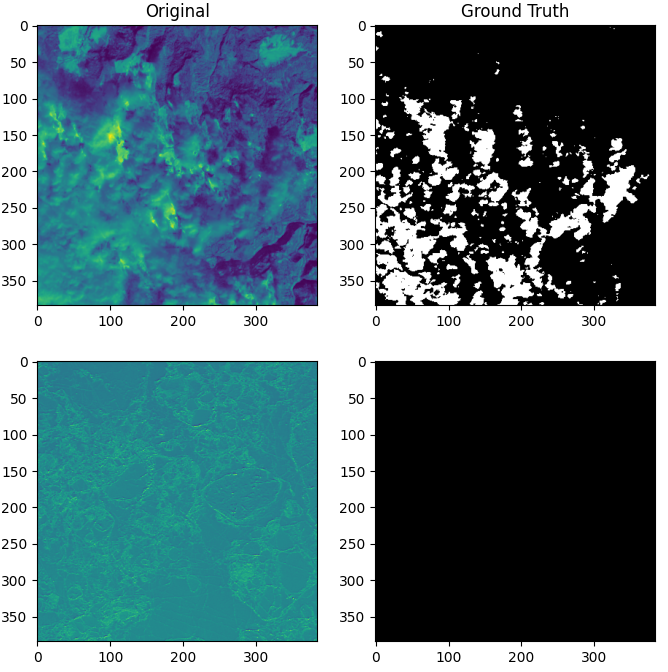
\includegraphics[scale=0.3]{images/hard.png}
    \caption{Example for challenging train images}
    \label{hard}
\end{figure}
\newpage
\subsection{Cloud Detection Algorithm}
Deep learning is a machine learning discipline that focuses on training artificial neural networks to recognize information and make predictions. It utilizes algorithms that can identify patterns and extract relevant information from large datasets. Deep learning models are designed to learn hierarchical structures in data by gradually acquiring more complex and abstract features. This learning process, known as training, involves adjusting the internal parameters of the neural network based on input data and desired output. The key component of deep learning is the artificial neural network, which consists of multiple layers of interconnected nodes. Each node performs computations and shares the results with other nodes in the network. The connections between nodes, represented by weights, are adjusted during training to optimize the network's performance.

In the context of image segmentation, a project was created using a U-Net-based software implementation of a Convolutional Neural Network. U-Net is a popular deep learning architecture known for its effectiveness in image segmentation tasks. Its U-shaped structure, consisting of an encoder and decoder network, enables efficient feature extraction and spatial information reconstruction.

The encoder network, similar to a convolutional neural network, employs convolutional and pooling layers to extract high-level features and capture context from input images. This reduces the spatial dimensions and increases the number of feature channels. On the other hand, the decoder network utilizes upsampling, concatenation operations, and convolutional layers to improve spatial resolution and generate a segmentation map. It combines feature maps and enhances spatial resolution to provide precise localization information. U-Net incorporates skip connections that connect corresponding levels of the encoder and decoder networks.

The final layer of the U-Net architecture consists of a 1x1 convolutional layer followed by a softmax activation function. This layer produces a pixel-by-pixel prediction probability map, where each pixel represents the likelihood of a particular class being present in the image.

The represantation of the U-NET Architecture is given below Figure \ref{unet}.
\begin{figure}[!htbp]
    \centering
    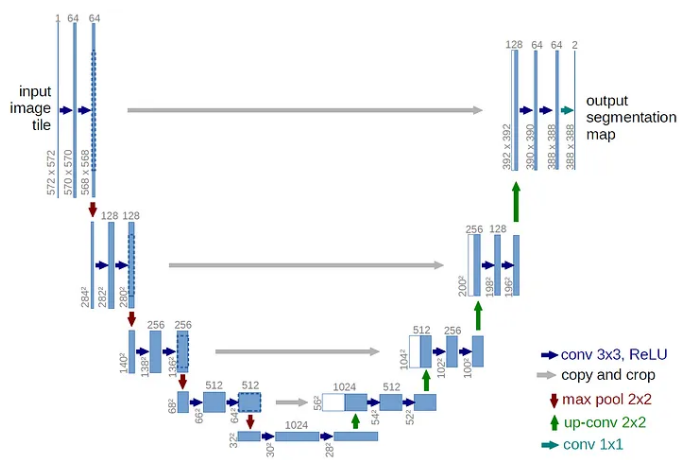
\includegraphics[scale=0.3]{images/unet.png}
    \caption{U-NET Architecture}
    \label{unet}
\end{figure}

The model is created using a collection of cloud pictures and ground truth masks supplied by the hub library. The code offers features for data loading and preprocessing, model definition and training, likewise performance evaluation on a test set. The Adam optimizer and the binary cross-entropy loss function are used to optimize the model. Evaluation metrics such as precision, recall, accuracy and mean Intersection over Union are utilized to assess the model's performance. During the training, checkpoints are implemented to store the optimal weights based on validation performance. Finally, the trained model is applied to forecast segmentation predictions on a test set of images.

The algorithm patterns are represented by the block diagram shown in Figure \ref{block}.

\begin{figure}[!htbp]
    \centering
    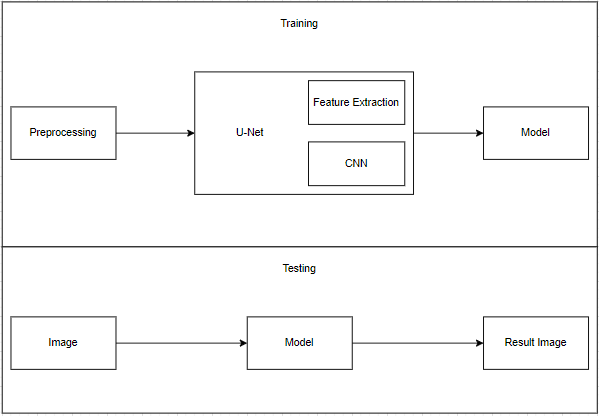
\includegraphics[scale=0.5]{images/blok_diyagram.png}
    \caption{Block Diagram}
    \label{block}
\end{figure}


\section{Experimental Results}

The Landsat 8 dataset contains 5154 images. The model was trained with 4124 random images and it was tested with 515 random images in the dataset. The performance measuring criterias are 'accuracy', 'precision', 'recall', 'IOU' and 'loss function' for the model's evaluation. 

Several experiments were carried out to determine the best functions and parameters for training and testing the model with Landsat 8 data. An owerview of the experiments and their results are provided below:

\begin{itemize}
    \item \textbf{U-Net Architecture Transformation:}\\
    
        The U-Net design was updated by adding an extra convolution function to each of the initial U-Net function's ten convolution layers. In this modification, the first convolution function received the result from the previous layer, while the second convolution function took the convoluted layer as a parameter. The new U-Net architecture was employed for both model training and testing, utilizing a dataset of 100 images. The results demonstrated that the Intersection over Union value decreased from 0.30 to 0.23, while the accuracy increased from 0.54 to 0.76.
        \\
    \item \textbf{Modifying Parameters in the U-Net Architecture:}\\
    
        In the U-Net design, the convolution function contains numerous hyperparameters, one of which is "kernel size." The kernel size is the size of the iterating window over the image during the convolution operation.

        The size of the kernel influences the information acquired by the convolutional layer. Larger kernel sizes can capture more global information, whereas lower kernel sizes can hold more local details.

        Two U-Net designs were trained and evaluated to identify the optimal kernel size for a specific set of data. One architecture used a kernel size of 3, while the other used a kernel size of 5.
        
        Increasing the kernel size from 3 to 5 resulted in a modest improvement in the Intersection over Union value, which improved from 0.30 to 0.31. Yet, there was a minor drop in accuracy, which decreased from 0.54 to 0.53.
        
        These findings indicate that the kernel size chosen might have a minor impact on the performance of the U-Net model, and it is critical to evaluate the trade-off between capturing global information and conserving local features when picking the kernel size for a specific dataset.
        \\
    \item \textbf{Modifying Optimization:}\\
        
        In the U-Net model, the compile function is used to prepare the model for training. There are three parameters required: optimizer, loss, and metrics.

        The optimizer is an optimization technique that determines how the weights of the model are changed during training. One of the optimizer's key parameters is the "learning rate." The learning rate is a hyperparameter that determines the size of the steps used to update the model's weights during training. It has an effect on how quickly or slowly the model learns from training data. A lower learning rate provides greater stability and the possibility of optimal solutions, whereas a higher learning rate allows for faster convergence.
        
        Three U-Net topologies were trained and tested to identify the best learning rate for a given dataset. Each architecture employed a distinct learning rate: 1e-3, 1e-4, and 1e-6.
        
        The results revealed that a learning rate of 1e-6 was insufficient for the model. With this learning rate, the precision and recall scores were approximately zero, indicating poor performance. Learning rates of 1e-3 and 1e-4, on the other hand, were more appropriate for the model. The IOU (Intersection Over Union) values obtained were 0.33 and 0.30, with corresponding accuracies of 0.55 and 0.54.
        
        These findings emphasize the significance of choosing an adequate learning rate while training the U-Net model. Both 1e-3 and 1e-4 performed better than the extremely low learning rate of 1e-6, demonstrating the importance of establishing the correct balance between learning speed and accuracy.
        \\
        \\
    \item \textbf{Modifying Compile Parameters:}\\
        \\
        The compile function in the U-Net model is used to prepare the model for training. Three parameters are required: optimizer, loss, and metrics.

        Loss function is the function that calculates the discrepancy between the ground truth and the predicted output of the model. The evolution metric is a parameter used to monitor the model's performance throughout training and testing. The accuracy metric is the most commonly used. It calculates the percentage of correctly predicted classes out of all samples for each sample. The binary accuracy metric computes correct predicted labels from all samples. 

        Four different compile functions were used for training and testing to determine the best compile parameters for a specific dataset. Binary cross entropy and dice loss functions were among the loss functions considered. Similarly, the metrics chosen included accuracy metrics and binary accuracy metrics. The goal of experimenting with different combinations of these four parameters was to find the compile function that produced the best results for the given dataset.

        The results showed that using the dice loss function and binary accuracy metric produced the highest IOU and accuracy values. In particular, the IOU value for the given dataset was 0.76, while the accuracy was 0.84.
\end{itemize}

All examination outcomes demonstrated the optimal U-Net architecture and compile function parameters. The features and parameters were determined after thorough examinations. The learning rate parameter in the optimization function was specifically set to "1e -4," while the kernel size was set at 3. Convolution layers were also implemented to the U - Net function. One of the compile function's parameters, the loss function, was set to the dice loss function. Similarly, the compile function's evaluation metric parameter was set to the binary accuracy metric. As a result, significant improvements in the acquired findings were pointed out.


The accuracy of the training and evolution is 0.91. The result outcomes after evaluation of the model are shown below in Figure \ref{res1} and Figure \ref{res2}.

\begin{figure}[htp]
    \centering
    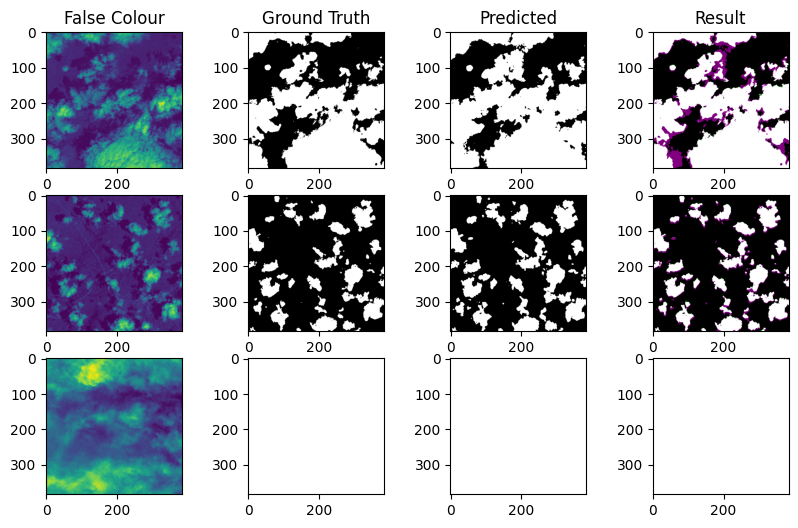
\includegraphics[width=8cm]{images/result1.png}
    \caption{Result Table 1}
    \label{res1}
\end{figure}

\begin{figure}[htp]
    \centering
    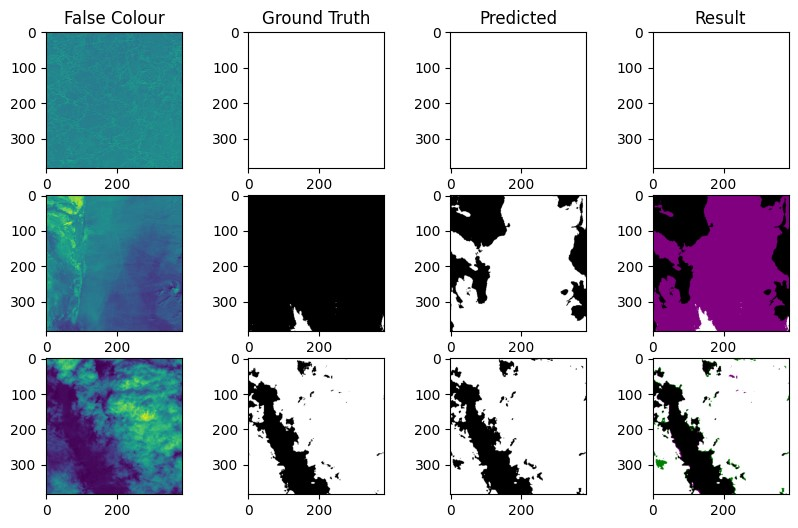
\includegraphics[width=8cm]{images/result2.png}
    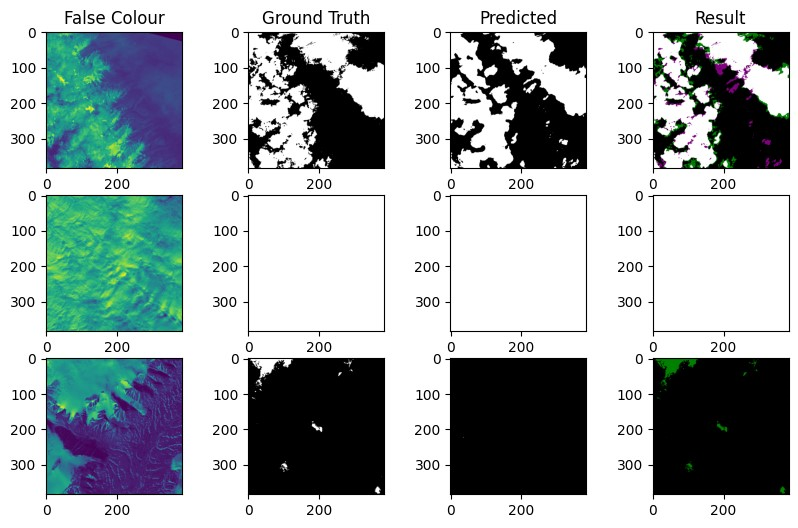
\includegraphics[width=8cm]{images/result3.png}
    \caption{Result Table 2}
    \label{res2}
\end{figure}

The success measurements obtained from training and evaluating the model are provided in Table \ref{resultTable}.
\begin{table}[!htp]

    \begin{tabular}{ |p{6cm}||p{2cm}|}
     \hline
     \multicolumn{2}{|c|}{Performance Criteria - Value} \\
     \hline
     Performance Criteria & Value\\
     \hline
     \hline
     IOU     &   0.8305\\
     \hline
     Precision   &     0.9309\\
     \hline
     Recall  &  0.9056\\
     \hline
     Binary Accuracy       &     0.9162\\
     \hline
     Loss &   0.2952\\
     \hline
    \end{tabular}

    \caption{Performance Criteria - Value}
    \label{resultTable}
\end{table}

\section{Performance Analysis}
4124 random images was employed in training, 515 random images was employed in validation and 515 random images was employed in testing process. The performance measuring criterias are 'accuracy', 'precision', 'recall', 'IOU' and 'loss function' for the model's evaluation. 

The checkpoint callback is utilized during training, and the model is trained on a train dataset for 20 epochs while utilizing a different validation dataset  for validation. When the model gets its best IOU score on the validation data, the weights will be saved.

While training the model, the CPU performance is shown in below Figure \ref{performance_cpu}. 
\begin{figure}[!htbp]
    \centering
    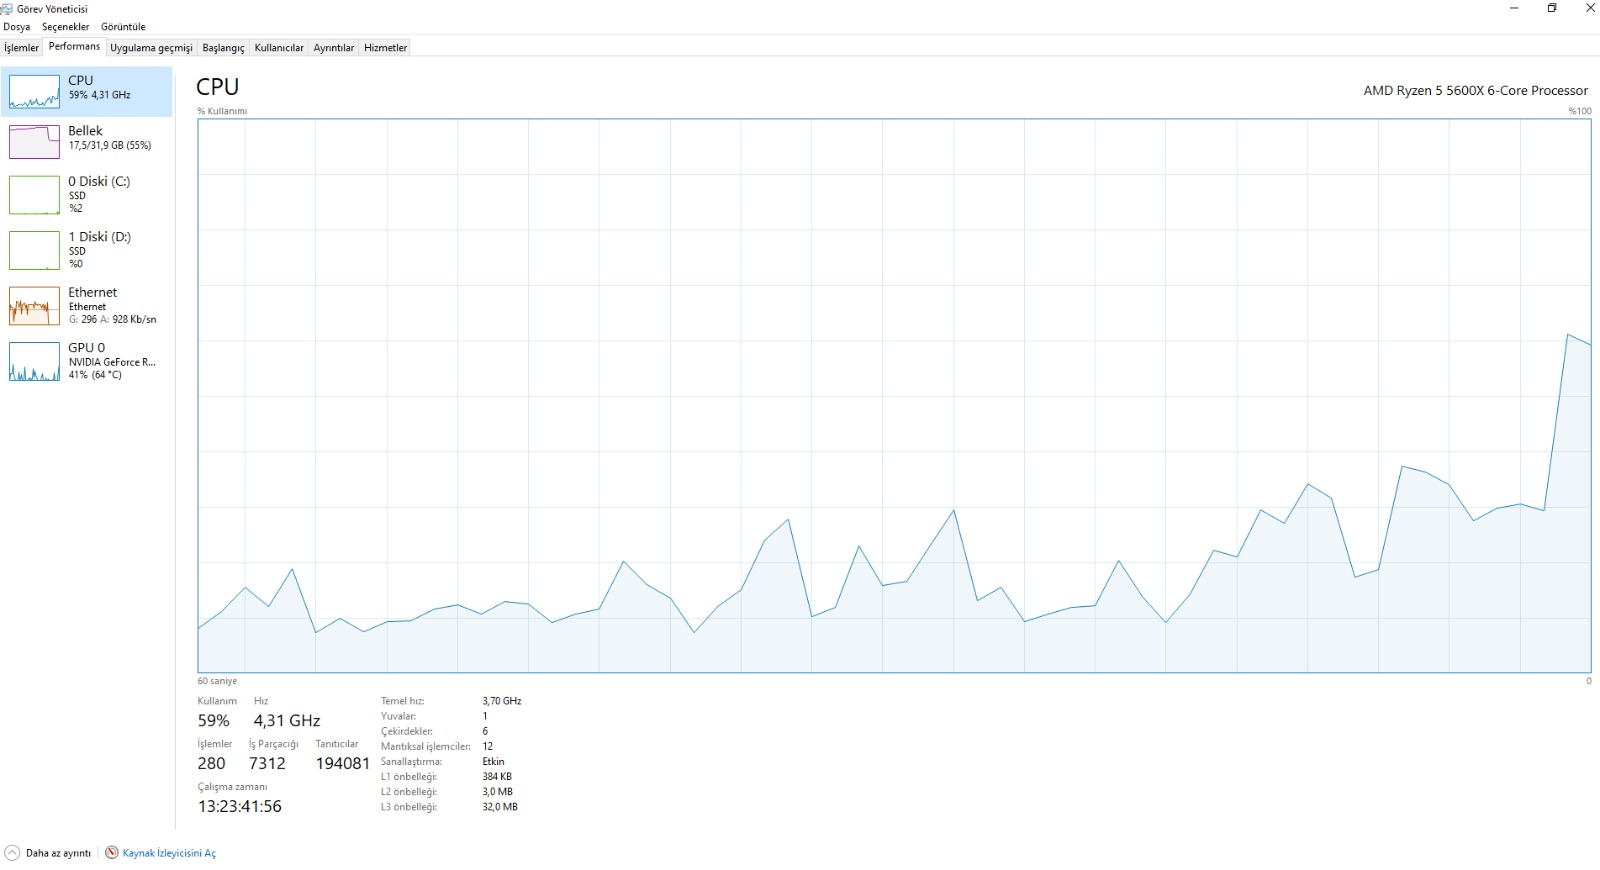
\includegraphics[scale=0.125]{images/performance_cpu.jpeg}
    \caption{CPU Usage}
    \label{performance_cpu}
\end{figure}

While training the model, the memory performance is shown in below Figure \ref{performance_memory}. 
\begin{figure}[!htbp]
    \centering
    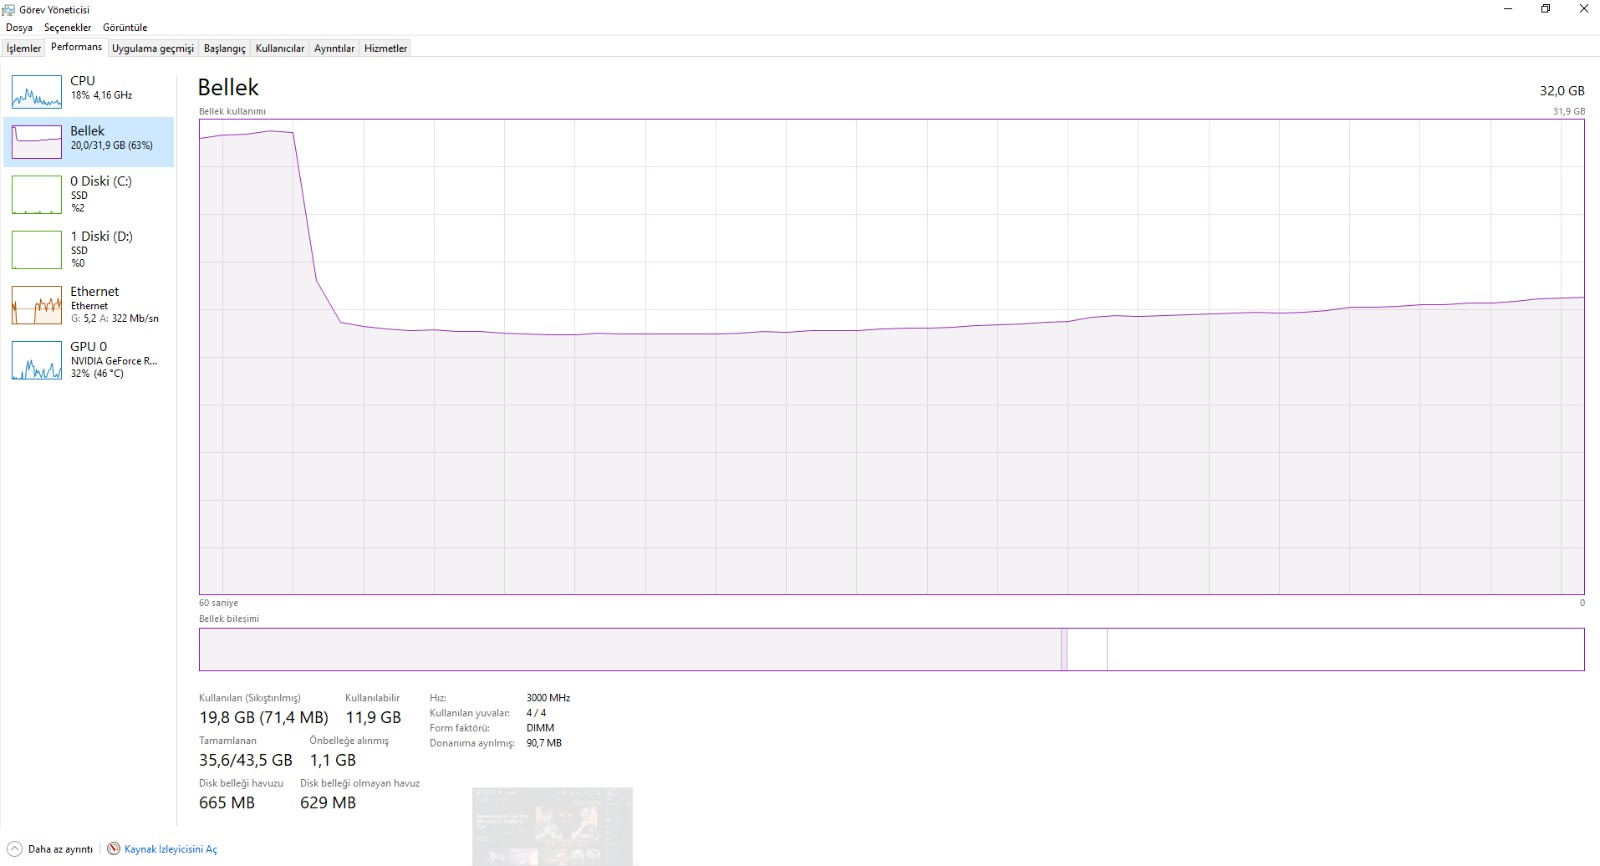
\includegraphics[scale=0.125]{images/performance_memory.jpeg}
    \caption{Memory Usage}
    \label{performance_memory}
\end{figure}

While training the model with, the GPU performance is shown in below Figure \ref{performance_gpu}. 
\begin{figure}[!htbp]
    \centering
    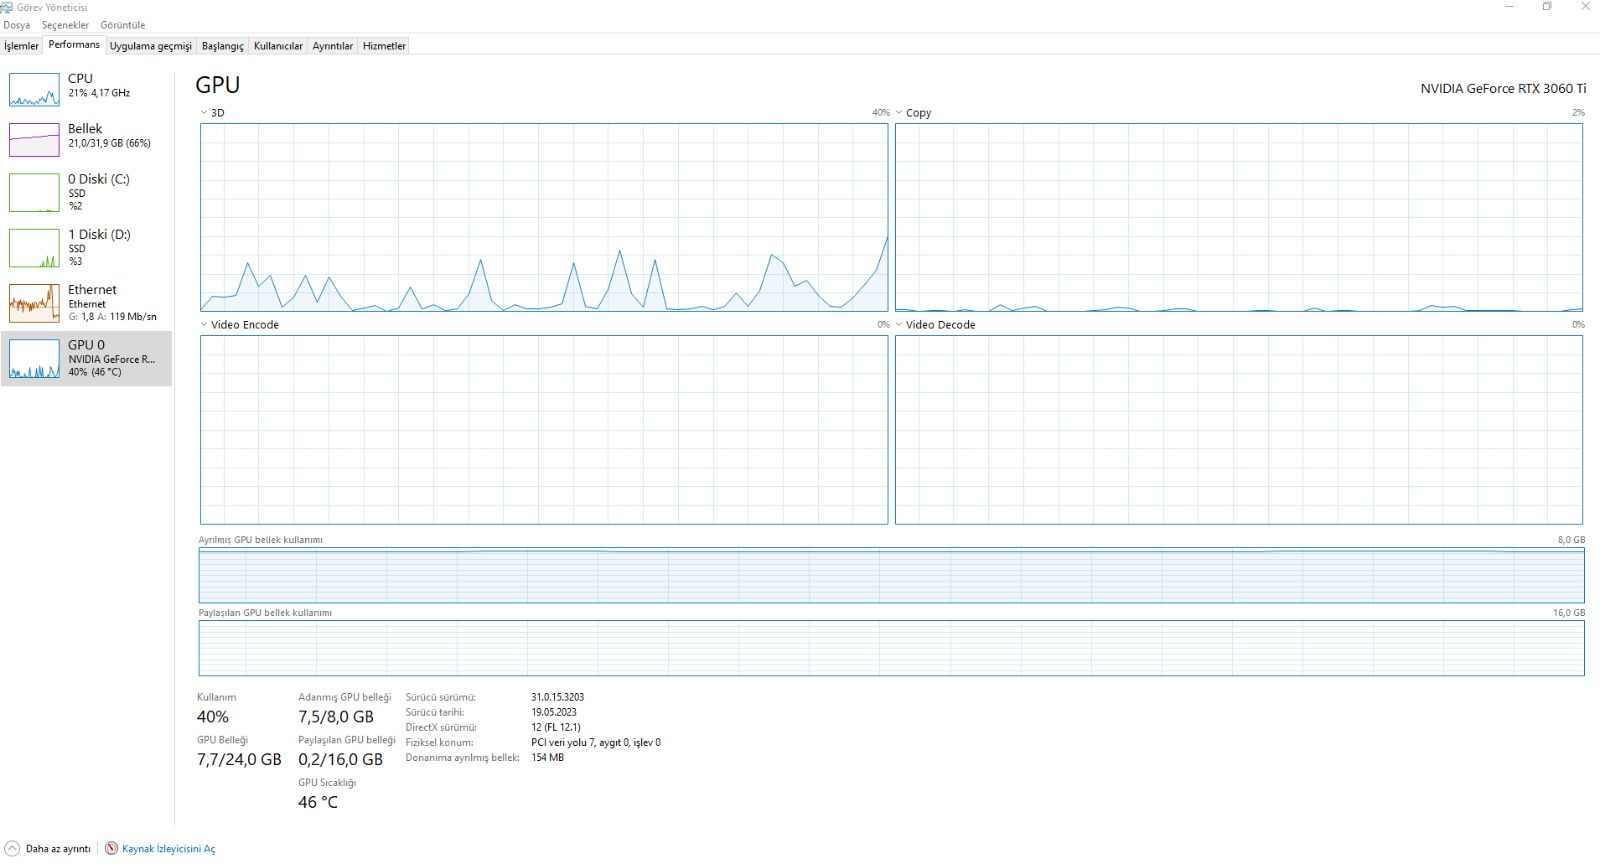
\includegraphics[scale=0.125]{images/performance_gpu.jpeg}
    \caption{GPU Usage}
    \label{performance_gpu}
\end{figure}

\section{Conclusion}
The project focuses on development of a deep learning model that can recognize clouds in satellite images. The U-Net architecture, a convolutional neural network based method, is used to define the model. The Landsat 8 satellite imagery dataset was used to training and testing the model. The task of binary classification for cloud presence and absence was successfully handled by the model. Additionally, the model performed semantic segmentation to precisely identify cloud regions within the images.

The model produced good results in cloud detection from satellite images after intensive training over 20 epochs using IOU as the saving criterion. The accuracy value was reached at \%91. By leveraging the information provided by the model, the non-informative regions dominated by clouds can be efficiently filtered  before subjecting the imagery to further algorithmic processing. This contributes to enhancing the overall effectiveness and accuracy of information retrieval procedures utilizing satellite imagery.


\bibliographystyle{IEEEtran}
\bibliography{references}
% that's all folks
\end{document}










